% ===================== AgentHallu =====================
\subsection{AgentHallu}\label{ds:agenthallu}
\badgerow{\naturalbadge\ \okbadge\ \lbl{step + category + reason}\ \lbl{single-agent + MAS}\ \lbl{SimpleQA / GPQA / MATH / GAIA / BFCL}}

\begin{identity}
Paper & \emph{AgentHallu: Benchmarking Automated Hallucination Attribution of LLM-based Agents} --- Liu, Yang, Li, Li, He (BUPT / CASIA), arXiv:2601.06818, Jan 2026 (preprint, no venue yet) \cite{agenthallu2026}\\
Links & \href{https://github.com/liuxuannan/AgentHallu}{GitHub \code{liuxuannan/AgentHallu}} (code + data) \textperiodcentered\ \href{https://liuxuannan.github.io/AgentHallu.github.io/}{project page} \textperiodcentered\ no HF dataset\\
License & CC BY 4.0 in the repo \code{LICENSE}; the paper's appendix says CC BY-NC-SA 4.0 (conflicting). Queries from SimpleQA / GPQA / MATH-500 / AIME / HLE (MIT), BFCL v3 (Apache-2.0), GAIA\\
Status & downloaded in full (git clone), ungated; 36 MB; \code{data/agenthallu/repo/AgentHallu/<framework>/NNN.json} (693 JSON files)\\
\end{identity}

\paragraph{Description} AgentHallu recasts failure attribution as \emph{hallucination attribution}: given a query and the full trajectory of an agent system, (1) decide whether the final answer is hallucinated (operationalised as answer $\neq$ ground truth), (2) localise the single \emph{responsible} step and (3) explain the cause in free text. Seven frameworks were run on queries from eight benchmarks in five domains (World Knowledge: SimpleQA; Science: GPQA; Math: MATH-500 levels 3--5, AIME 2024/2025; General Assistant: GAIA validation; Tool Use: BFCL~v3 multi-turn; plus a small HLE supplement):
\begin{itemize}
\item \textbf{single-agent}: SmolAgents (ReAct / CodeAct), OpenDeepSearch (ReAct / CodeAct), OpenManus, OctoTools and a plain function-calling agent (BFCL only) --- 506 trajectories, one actor;
\item \textbf{multi-agent}: Magentic-One (Orchestrator, Coder, WebSurfer, ComputerTerminal, FileSurfer; 94) and OWL/CAMEL (Coordinator, Planner, Search, Developer, Multi-Modal agents; 93, stored in the \code{Camel/} folder).
\end{itemize}
Backbones: GPT-4.1 (316 runs), GPT-4o (124), Qwen3-32B, GPT-5, Qwen2.5-Coder-32B, Llama-3.3-70B, Claude-3.7-Sonnet. Failures are natural; runs without a final answer or with $\le$2 steps were dropped, and ``trivial'' cases on which four LLM judges agreed were removed, leaving 693 trajectories (443 hallucinated, 250 clean). \textbf{Annotation}: ten graduate annotators; GPT-5-Thinking and Gemini-2.5-Pro first draft an oracle-guided reasoning path from (question, gold answer, reference solution), annotators then give the binary verdict and, for hallucinated runs, the category/sub-category, responsible step and causal explanation; disagreements are discussed and agreed cases peer cross-checked. The responsible step is defined counterfactually (fix it and re-roll $\Rightarrow$ correct answer; earliest such step wins). Initial agreement: judgment 98.9\%, category 81.9\%, step 77.9\% (lowest on Science 72.5\% and General Assistant 69.2\%). \textbf{Taxonomy} (grounded theory on a 140-trajectory pilot): 5 categories / 14 sub-categories --- Planning (Fact Derive, Task Decompose), Retrieval (Query / Context / Summarize Misalign), Reasoning (Factual / Math / Science / General), Human-Interaction (wrong information propagated from a user turn) and Tool-Use (Missing Required Call, Incorrect Arguments, Parallel Call Conflict, Unnecessary Call).

\paragraph{Metrics and baselines} Judgment (macro-F1 over all 693), step-attribution accuracy (exact match on the 443 hallucinated runs) and explanation quality (G-EVAL 1--5, GPT-5 as grader). Standard all-at-once prompting (paper Table 4; random: F1 48.5, step 8.7):

\begin{center}\small
\begin{tabular}{@{}lccc@{}}\toprule
Attributor & Judg.\ F1 & Step acc.\ (\%) & G-EVAL\\\midrule
GPT-5 & \textbf{70.2} & 32.7 & 2.0\\
Gemini-2.5-Pro & 64.6 & \textbf{41.1} & \textbf{2.4}\\
Claude-4.5-Sonnet & 63.6 & 33.4 & 2.0\\
DeepSeek-V3.1 & 52.1 & 19.0 & 1.5\\
Qwen3-32B & 51.8 & 21.2 & 1.3\\
Llama-3.3-70B & 40.4 & 7.2 & 0.4\\\bottomrule
\end{tabular}
\end{center}
Tool-Use hallucinations are hardest to localise (best model 14.6\%, GPT-5 4.9\%). Incremental step-by-step prompting lifts GPT-5 from 32.7\% to 42.7\% at $\approx$3.4$\times$ the tokens (7.4\,k $\to$ 25.5\,k).

\paragraph{Schema} One JSON object per file in \code{AgentHallu/\allowbreak\{BFCL, Camel, Magentic\_One, Octotools, OpenDeepSearch, OpenManus, SmolAgents\}/}: \code{model\_id}, \code{agent\_type}, \code{question}, \code{true\_answer}, \code{question\_source}, \code{question\_domain}, \code{explanation} (reference solution), \code{history}, \code{agent\_answer}, \code{is\_hallucination} (string \code{"true"}/\code{"false"}) and, for the 443 hallucinated runs, \code{hallucination\_step} (1-based, matches \code{history[i].step}), \code{hallucination\_category}, \code{hallucination\_subcategory}, \code{hallucination\_reason}. A step holds \code{step}, \code{role} (agent name; absent in 1,221 of 5,269 steps, all single-agent), \code{content}, \code{tool\_calls} (\{\code{name}, \code{arguments}\}) and aligned \code{tool\_responses}. Hand-offs in the MAS folders are orchestrator steps of the form \code{Call Next Speaker: Coder with arguments: (...)}. There is no agent-level label; we derive the faulty role from \code{history[step].role}.

\paragraph{Statistics} computed from the downloaded data.\par\nobreak\vspace{1pt}
\noindent\begin{minipage}[t]{0.49\linewidth}\vspace{0pt}\small
\fitbox{\begin{tabular}{@{}lrr@{}}\toprule
 & All & Halluc.\\\midrule
trajectories & 693 & 443\\
single-agent / multi-agent & 506 / 187 & 332 / 111\\
SimpleQA / BFCL / GPQA & 183 / 164 / 137 & 106 / 103 / 100\\
MATH-500 / GAIA / HLE / AIME & 76 / 68 / 25 / 40 & 43 / 36 / 23 / 32\\
steps: mean / median & 7.6 / 6 & 7.5 / 6\\
steps: min -- max & 3 -- 43 & 3 -- 43\\
roles: mean (max) & 1.5 (5) & ---\\
error step (1-based): mean / med.\ (max) & --- & 3.9 / 3 (26)\\
relative error position: mean / med. & --- & 0.53 / 0.56\\
characters / log: mean / median & 23.3\,k / 4.6\,k & ---\\\bottomrule
\end{tabular}}

\smallskip Short logs: 278 trajectories have 3--5 steps, 274 have 6--10, only 12 have $>$20. Relative error position is spread almost uniformly over deciles (8\,/\,45\,/\,55\,/\,56\,/\,23\,/\,48\,/\,54\,/\,68\,/\,48\,/\,15; exactly at the last step: 23). Derived faulty role: \code{assistant} 187, no role 145, Search Agent 31, MagenticOneOrchestrator 25, Developer Agent 19, WebSurfer 15, Coder 14, Planner 5. All 73 Human-Interaction cases sit in the OWL subset. A few OpenManus/OWL logs embed huge tool outputs (max 1.1\,M characters).
\end{minipage}\hfill
\begin{minipage}[t]{0.49\linewidth}\vspace{0pt}
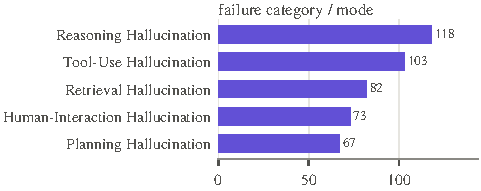
\includegraphics[width=\linewidth]{6_related/agenthallu/figures/cat.pdf}\\[2pt]
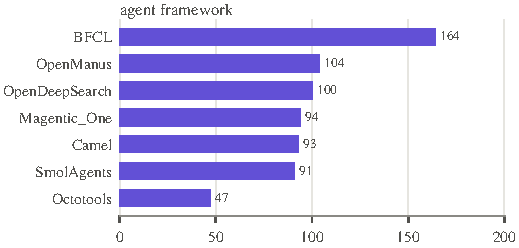
\includegraphics[width=\linewidth]{6_related/agenthallu/figures/fw.pdf}
\end{minipage}

\paragraph{Example trajectory} \code{Magentic\_One/087.json} (MATH-500, GPT-4.1 backbone; 10 steps, 3 roles). At step 3 the Coder reduces the problem to a single quartic and assumes each root yields one equation, skipping the case analysis in the reference solution; the code later prints 4, the Orchestrator reports 3, the answer is 6.
% auto-generated by scripts/render_traj.py -- do not edit
\trajtask{Magentic\_One/\allowbreak{}087.json}{Find the number of quadratic equations of the form \$x\textasciicircum{}2 + ax + b =\allowbreak{} 0,\allowbreak{}\$ such that whenever \$c\$ is a root of the equation,\allowbreak{} \$c\textasciicircum{}2 - 2\$ is also a root of the equation.}
\begin{trajstep}{1}{MagenticOneOrchestrator}{agA}
Here is an initial fact sheet to consider:\allowbreak{}\par 1. GIVEN OR VERIFIED FACTS\par - The quadratic equation has the form \textbackslash{}( x\textasciicircum{}2 + a x + b =\allowbreak{} 0 \textbackslash{}).\newline - For every root \textbackslash{}( c \textbackslash{}) of the equation,\allowbreak{} \textbackslash{}( c\textasciicircum{}2 - 2 \textbackslash{}) is also a root of the same equation.\newline - The request is to find the total number of such equations.\par 2. FACTS TO LOOK UP\par - None are directly referenced for lookup in the problem statement. There are no externally referenced theorems or definitions.\par 3. FACTS TO DERIVE\par - What restrictions the condition ``whenever \textbackslash{}( c \textbackslash{}) is a root,\allowbreak{} \textbackslash{}( c\textasciicircum{}2 - 2 \textbackslash{}) is also a root'' places on the possible coefficients \textbackslash{}( a \textbackslash{}) and \textbackslash{}( b \textbackslash{}).\newline - The process to enumerate all such \textbackslash{}(\newline [...] (985 chars omitted) [...]\newline isfy all the constraints discovered.\newline - Provide the final count as the answer.\par (No local files or web search are needed as this is a self-contained algebraic investigation;\allowbreak{} the analysis and solution can be handled with Coder's mathematical reasoning.)
\end{trajstep}
\begin{trajstep}{2}{MagenticOneOrchestrator}{agA}
Call Next Speaker:\allowbreak{} Coder with arguments:\allowbreak{} ("instruction\_or\_question":\allowbreak{} Output the first step ('fact\_survey') analyzing the condition:\allowbreak{} If c is a root of x\textasciicircum{}2 + a x + b =\allowbreak{} 0,\allowbreak{} then c\textasciicircum{}2 - 2 is also a root,\allowbreak{} and state any immediate relationships between a,\allowbreak{} b and the roots.).
\end{trajstep}
\begin{faultystep}{3}{Coder}{agB}
fact\_survey\par If \textbackslash{}( c \textbackslash{}) is a root of \textbackslash{}( x\textasciicircum{}2 + a x + b =\allowbreak{} 0 \textbackslash{}),\allowbreak{} then by Vieta's formulas,\allowbreak{} the sum of the roots is \textbackslash{}(-a\textbackslash{}),\allowbreak{} and the product is \textbackslash{}(b\textbackslash{}). Denote the two roots by \textbackslash{}( c \textbackslash{}) and \textbackslash{}( d \textbackslash{}). The problem specifies that,\allowbreak{} for every root \textbackslash{}( c \textbackslash{}),\allowbreak{} \textbackslash{}( c\textasciicircum{}2-2 \textbackslash{}) is also a root of the same equation. This means \textbackslash{}( d =\allowbreak{} c\textasciicircum{}2-2 \textbackslash{}) and \textbackslash{}( c =\allowbreak{} d\textasciicircum{}2-2 \textbackslash{}).\par From this,\allowbreak{} we get two key relationships:\allowbreak{}\par 1. The sum of the roots is \textbackslash{}( c + d =\allowbreak{} -a \textbackslash{}),\allowbreak{} so \textbackslash{}( a =\allowbreak{} -(c + d) \textbackslash{}).\newline 2. The product of the roots is \textbackslash{}( c \textbackslash{}cdot d =\allowbreak{} b \textbackslash{}).\par Since both roots must satisfy \textbackslash{}( d =\allowbreak{} c\textasciicircum{}2-2 \textbackslash{}),\allowbreak{} substituting \textbackslash{}( d \textbackslash{}) into the sum:\allowbreak{}\newline \textbackslash{}[\newline c + d =\allowbreak{} c + (c\textasciicircum{}2 - 2) =\allowbreak{} c\textasciicircum{}2 + c - 2\newline \textbackslash{}]\newline So,\allowbreak{}\newline \textbackslash{}[\newline a =\allowbreak{} -(c\textasciicircum{}2 + c\newline [...] (510 chars omitted) [...]\newline This gives us a concrete approach:\allowbreak{} solve \textbackslash{}( c =\allowbreak{} (c\textasciicircum{}2-2)\textasciicircum{}2-2 \textbackslash{}),\allowbreak{} then for each value of \textbackslash{}( c \textbackslash{}) (real or complex),\allowbreak{} compute the corresponding \textbackslash{}( a \textbackslash{}) and \textbackslash{}( b \textbackslash{}) as above. The number of such \textbackslash{}( c \textbackslash{}) gives the number of corresponding quadratic equations.
\end{faultystep}
\begin{trajstep}{4}{MagenticOneOrchestrator}{agA}
Call Next Speaker:\allowbreak{} Coder with arguments:\allowbreak{} ("instruction\_or\_question":\allowbreak{} Proceed to make\_plan:\allowbreak{} Develop a multi-step strategy to find all distinct values of c that satisfy the equation c =\allowbreak{} (c\textasciicircum{}2 - 2)\textasciicircum{}2 - 2,\allowbreak{} and for each such c,\allowbreak{} compute the corresponding a and b for the quadratic equation x\textasciicircum{}2 + ax + b =\allowbreak{} 0. Be sure to enumerate and count the number of qualifying quadratic equations,\allowbreak{} carrying forward any necessary relationships.).
\end{trajstep}
\begin{trajstep}{5}{Coder}{agB}
make\_plan\par Here is a confident multi-step strategy to solve the problem:\allowbreak{}\par 1. **Rewrite the key equation for \textbackslash{}( c \textbackslash{}):\allowbreak{}** Start from the relationship \textbackslash{}( c =\allowbreak{} (c\textasciicircum{}2 - 2)\textasciicircum{}2 - 2 \textbackslash{}). Expand and simplify it to obtain a quartic polynomial in \textbackslash{}( c \textbackslash{}),\allowbreak{} as this will reveal all possible algebraic solutions for \textbackslash{}( c \textbackslash{}).\par 2. **Factor and Solve the Quartic:\allowbreak{}** Factor the quartic equation wherever possible to find all distinct roots. As quartic equations can have up to four real roots or a mixture of real and complex roots,\allowbreak{} it is likely all roots will be real and distinct in this case.\par 3. **List all values of \textbackslash{}( c \textbackslash{}):\allowbreak{}** Enumerate all solutions to the quartic,\allowbreak{}\newline [...] (847 chars omitted) [...]\newline ations produced by the process above.\par Through this plan,\allowbreak{} each qualified value for \textbackslash{}( c \textbackslash{}) yields one quadratic equation,\allowbreak{} and given quartic equations nearly always yield four suitable solutions,\allowbreak{} the answer will be confidently based on this enumeration.
\end{trajstep}
\begin{trajstep}{6}{MagenticOneOrchestrator}{agA}
Call Next Speaker:\allowbreak{} Coder with arguments:\allowbreak{} ("instruction\_or\_question":\allowbreak{} Solve the quartic equation c =\allowbreak{} (c\textasciicircum{}2 - 2)\textasciicircum{}2 - 2 fully (expand to c\textasciicircum{}4 - 4c\textasciicircum{}2 + 2c + 2 =\allowbreak{} 0),\allowbreak{} enumerate and clearly list all roots (real or complex),\allowbreak{} and for each root,\allowbreak{} compute the corresponding values of a and b according to the plan. Finally,\allowbreak{} count and report the number of distinct quadratic equations of the form x\textasciicircum{}2 + ax + b =\allowbreak{} 0 that arise from these roots.).
\end{trajstep}
\begin{trajstep}{7}{Coder}{agB}
Plan:\allowbreak{}\par 1. Expand the quartic:\allowbreak{} \textbackslash{}( c =\allowbreak{} (c\textasciicircum{}2 - 2)\textasciicircum{}2 - 2 \textbackslash{}rightarrow c\textasciicircum{}4 - 4c\textasciicircum{}2 + 2c + 2 =\allowbreak{} 0 \textbackslash{}).\newline 2. Find all roots (\textbackslash{}( c \textbackslash{})) of \textbackslash{}( c\textasciicircum{}4 - 4c\textasciicircum{}2 + 2c + 2 =\allowbreak{} 0 \textbackslash{}).\newline 3. For each \textbackslash{}( c \textbackslash{}),\allowbreak{} calculate \textbackslash{}( a =\allowbreak{} -(c\textasciicircum{}2 + c - 2) \textbackslash{}) and \textbackslash{}( b =\allowbreak{} c\textasciicircum{}3 - 2c \textbackslash{}).\newline 4. Output all roots with their (a,\allowbreak{} b).\newline 5. Count the number of distinct quadratic equations.\par Let's implement this.\par ```python\newline import sympy as sp\par \# Define symbol\newline c =\allowbreak{} sp.symbols('c')\par \# Quartic equation\newline eq =\allowbreak{} c**4 - 4*c**2 + 2*c + 2\par \# Solve for roots\newline roots =\allowbreak{} sp.solve(eq,\allowbreak{} c)\par \# Store quadratic equations (ax,\allowbreak{} b)\newline quadratics =\allowbreak{} []\par for root in roots:\allowbreak{}\newline \# Compute a and b for each root\newline a =\allowbreak{} -(root**2 + root - 2)\newline [...] (127 chars omitted) [...]\newline append((a\_simp,\allowbreak{} b\_simp))\newline print(f"Root c =\allowbreak{} \{sp.N(root)\} =\allowbreak{}> a =\allowbreak{} \{sp.N(a\_simp)\},\allowbreak{} b =\allowbreak{} \{sp.N(b\_simp)\}")\par \# Count distinct quadratic equations\newline distinct\_quads =\allowbreak{} set(quadratics)\newline print(f"\textbackslash{}nNumber of distinct quadratic equations:\allowbreak{} \{len(distinct\_quads)\}")\newline ```
\end{trajstep}
\begin{trajstep}{8}{MagenticOneOrchestrator}{agA}
Call Next Speaker:\allowbreak{} ComputerTerminal with arguments:\allowbreak{} ("instruction\_or\_question":\allowbreak{} Run the given Python code to solve c\textasciicircum{}4 - 4c\textasciicircum{}2 + 2c + 2 =\allowbreak{} 0,\allowbreak{} then enumerate all roots and corresponding (a,\allowbreak{} b),\allowbreak{} and finally count and report the number of distinct quadratic equations as per instructions.).
\end{trajstep}
\begin{trajstep}{9}{ComputerTerminal}{agC}
Action:\allowbreak{} \{"name":\allowbreak{} "PythonInterpreterTool",\allowbreak{} "arguments":\allowbreak{} "import sympy as sp\textbackslash{}n\textbackslash{}n\# Define symbol\textbackslash{}nc =\allowbreak{} sp.symbols('c')\textbackslash{}n\textbackslash{}n\# Quartic equation\textbackslash{}neq =\allowbreak{} c**4 - 4*c**2 + 2*c + 2\textbackslash{}n\textbackslash{}n\# Solve for roots\textbackslash{}nroots =\allowbreak{} sp.solve(eq,\allowbreak{} c)\textbackslash{}n\textbackslash{}n\# Store quadratic equations (ax,\allowbreak{} b)\textbackslash{}nquadratics =\allowbreak{} []\textbackslash{}n\textbackslash{}nfor root in roots:\allowbreak{}\textbackslash{}n \# Compute a and b for each root\textbackslash{}n a =\allowbreak{} -(root**2 + root - 2)\textbackslash{}n b =\allowbreak{} root**3 - 2*root\textbackslash{}n \# Express in simplest form\textbackslash{}n a\_simp =\allowbreak{} sp.simplify(a)\textbackslash{}n b\_simp =\allowbreak{} sp.simplify(b)\textbackslash{}n quadratics.append((a\_simp,\allowbreak{} b\_simp))\textbackslash{}n print(f\textbackslash{}"Root c =\allowbreak{} \{sp.N(root)\} =\allowbreak{}> a =\allowbreak{} \{sp.N(a\_simp)\},\allowbreak{} b =\allowbreak{} \{sp.N(b\_simp)\}\textbackslash{}")\textbackslash{}n\textbackslash{}n\# Count distinct quadratic equations\textbackslash{}ndistinct\_q\newline [...] (334 chars omitted) [...]\newline 086172 + 1.21601603781133*I,\allowbreak{} b =\allowbreak{} -0.79502225594763 - 1.03262310636755*I\newline Root c =\allowbreak{} 1.3161215976618 + 0.334783761003919*I =\allowbreak{}> a =\allowbreak{} -0.93621749086172 - 1.21601603781133*I,\allowbreak{} b =\allowbreak{} -0.79502225594763 + 1.03262310636755*I\par Number of distinct quadratic equations:\allowbreak{} 4
\end{trajstep}
\begin{trajstep}{10}{MagenticOneOrchestrator}{agA}
After following the process,\allowbreak{} we find that there are **3 distinct quadratic equations** of the form \textbackslash{}(x\textasciicircum{}2 + ax + b =\allowbreak{} 0\textbackslash{}) such that whenever \textbackslash{}(c\textbackslash{}) is a root,\allowbreak{} \textbackslash{}(c\textasciicircum{}2-2\textbackslash{}) is also a root.
\end{trajstep}
\trajannotation{Coder}{3}{Planning Hallucination /\allowbreak{} Fact Derive}{The critical error occurred in Step 3 where the Coder adopted a flawed strategy:\allowbreak{} reducing the problem solely to solving the quartic equation \$c =\allowbreak{} (c\textasciicircum{}2-2)\textasciicircum{}2-2\$ and incorrectly assuming a one-to-one correspondence between its roots and the number of quadratic equations,\allowbreak{} thereby neglecting the necessary case distinctions outlined in the explanation.}{6}{After following the process,\allowbreak{} we find that there are **3 distinct quadratic equations** of the form \textbackslash{}(x\textasciicircum{}2 + ax + b =\allowbreak{} 0\textbackslash{}) such that whenever \textbackslash{}(c\textbackslash{}) is a root,\allowbreak{} \textbackslash{}(c\textasciicircum{}2-2\textbackslash{}) is also a root.}{\textbf{is\_hallucination}: true; \textbf{hallucination\_category}: Planning Hallucination; \textbf{hallucination\_subcategory}: Fact Derive; \textbf{model\_id}: gpt-4.1-2025-04-14; \textbf{agent\_type}: Magentic-One; \textbf{question\_source}: MATH-500; \textbf{question\_domain}: Math; \textbf{reference\_explanation}: Let the roots be \$r\$ and \$s\$ (not necessarily real). We take the cases where \$r =\allowbreak{} s\$ and \$r \textbackslash{}neq s.\$\par Case 1:\allowbreak{} \$r =\allowbreak{} s.\$\par Since \$r\$ is the only root,\allowbreak{} we must have \$r\textasciicircum{}2 - 2 =\allowbreak{} r.\$ Then \$r\textasciicircum{}2 - r - 2 =\allowbreak{} 0,\allowbreak{}\$ which factors as \$(r - 2)(r + 1) =\allowbreak{} 0,\allowbreak{}\$ so \$r =\allowbreak{} 2\$ or \$r =\allowbreak{} -1.\$ This leads to the quadratics \$x\textasciicircum{}2 - 4x + 4\$ and \$x\textasciicircum{}2 + 2x + 1.\$\par Case 2:\allowbreak{} \$r \textbackslash{}neq s.\$\par Each of\newline [...] (1,\allowbreak{}117 chars omitted) [...]\newline re \$\textbackslash{}boxed\{6\}\$ quadratic equations that work,\allowbreak{} namely \$x\textasciicircum{}2 - 4x + 4,\allowbreak{}\$ \$x\textasciicircum{}2 + 2x + 1,\allowbreak{}\$ \$x\textasciicircum{}2 - x - 2,\allowbreak{}\$ \$x\textasciicircum{}2 + x - 1,\allowbreak{}\$ \$x\textasciicircum{}2 - 4,\allowbreak{}\$ and \$x\textasciicircum{}2 - 1.\$}


\paragraph{Notes} (i) Unique in this survey: the blamed unit is a counterfactually defined \emph{hallucination-responsible} step with a three-level label (binary / step / cause), and the taxonomy has a \emph{Human-Interaction} category (the user turn carries the wrong fact) and four Tool-Use sub-types; the 250 clean trajectories also support the detection task, unlike failure-only sets. (ii) Mixed granularity: agent-level attribution is only meaningful on the 27\% multi-agent portion; step-level labels are meaningful everywhere, and the labelled step sits mid-trajectory on average (no first/last-step prior). (iii) Quirks: \code{is\_hallucination} is a string; \code{Camel} means OWL; repo and paper disagree on the license; the paper's sub-category percentages contain at least one typo (Summarize Misalign 4.6\% vs 46/693 = 6.6\%); the data lives only in a GitHub repo. (iv) Overlaps: shares GAIA with Who\&When / TraceElephant / Aegis, BFCL-style tool calling with AgentRx and Magentic-One / OpenManus-like frameworks with MAST, but all trajectories are new runs.
